\documentclass[11pt,]{article}
\usepackage{lmodern}
\usepackage{amssymb,amsmath}
\usepackage{ifxetex,ifluatex}
\usepackage{fixltx2e} % provides \textsubscript
\ifnum 0\ifxetex 1\fi\ifluatex 1\fi=0 % if pdftex
  \usepackage[T1]{fontenc}
  \usepackage[utf8]{inputenc}
\else % if luatex or xelatex
  \ifxetex
    \usepackage{mathspec}
  \else
    \usepackage{fontspec}
  \fi
  \defaultfontfeatures{Ligatures=TeX,Scale=MatchLowercase}
    \setmainfont[]{SF Pro Text Light}
\fi
% use upquote if available, for straight quotes in verbatim environments
\IfFileExists{upquote.sty}{\usepackage{upquote}}{}
% use microtype if available
\IfFileExists{microtype.sty}{%
\usepackage{microtype}
\UseMicrotypeSet[protrusion]{basicmath} % disable protrusion for tt fonts
}{}
\usepackage[margin=1in]{geometry}
\usepackage{hyperref}
\hypersetup{unicode=true,
            pdftitle={October 16 Notes},
            pdfauthor={Philosophy 444},
            pdfborder={0 0 0},
            breaklinks=true}
\urlstyle{same}  % don't use monospace font for urls
\usepackage{longtable,booktabs}
\usepackage{graphicx,grffile}
\makeatletter
\def\maxwidth{\ifdim\Gin@nat@width>\linewidth\linewidth\else\Gin@nat@width\fi}
\def\maxheight{\ifdim\Gin@nat@height>\textheight\textheight\else\Gin@nat@height\fi}
\makeatother
% Scale images if necessary, so that they will not overflow the page
% margins by default, and it is still possible to overwrite the defaults
% using explicit options in \includegraphics[width, height, ...]{}
\setkeys{Gin}{width=\maxwidth,height=\maxheight,keepaspectratio}
\IfFileExists{parskip.sty}{%
\usepackage{parskip}
}{% else
\setlength{\parindent}{0pt}
\setlength{\parskip}{6pt plus 2pt minus 1pt}
}
\setlength{\emergencystretch}{3em}  % prevent overfull lines
\providecommand{\tightlist}{%
  \setlength{\itemsep}{0pt}\setlength{\parskip}{0pt}}
\setcounter{secnumdepth}{0}
% Redefines (sub)paragraphs to behave more like sections
\ifx\paragraph\undefined\else
\let\oldparagraph\paragraph
\renewcommand{\paragraph}[1]{\oldparagraph{#1}\mbox{}}
\fi
\ifx\subparagraph\undefined\else
\let\oldsubparagraph\subparagraph
\renewcommand{\subparagraph}[1]{\oldsubparagraph{#1}\mbox{}}
\fi

%%% Use protect on footnotes to avoid problems with footnotes in titles
\let\rmarkdownfootnote\footnote%
\def\footnote{\protect\rmarkdownfootnote}

%%% Change title format to be more compact
\usepackage{titling}

% Create subtitle command for use in maketitle
\providecommand{\subtitle}[1]{
  \posttitle{
    \begin{center}\large#1\end{center}
    }
}

\setlength{\droptitle}{-2em}

  \title{October 16 Notes}
    \pretitle{\vspace{\droptitle}\centering\huge}
  \posttitle{\par}
    \author{Philosophy 444}
    \preauthor{\centering\large\emph}
  \postauthor{\par}
      \predate{\centering\large\emph}
  \postdate{\par}
    \date{16 October, 2019}

\usepackage{mathastext}
\usepackage{nicefrac}

\begin{document}
\maketitle

\hypertarget{subgame-and-nash-equilibrium}{%
\section{Subgame and Nash
Equilibrium}\label{subgame-and-nash-equilibrium}}

Consider this game, from Bonnano.

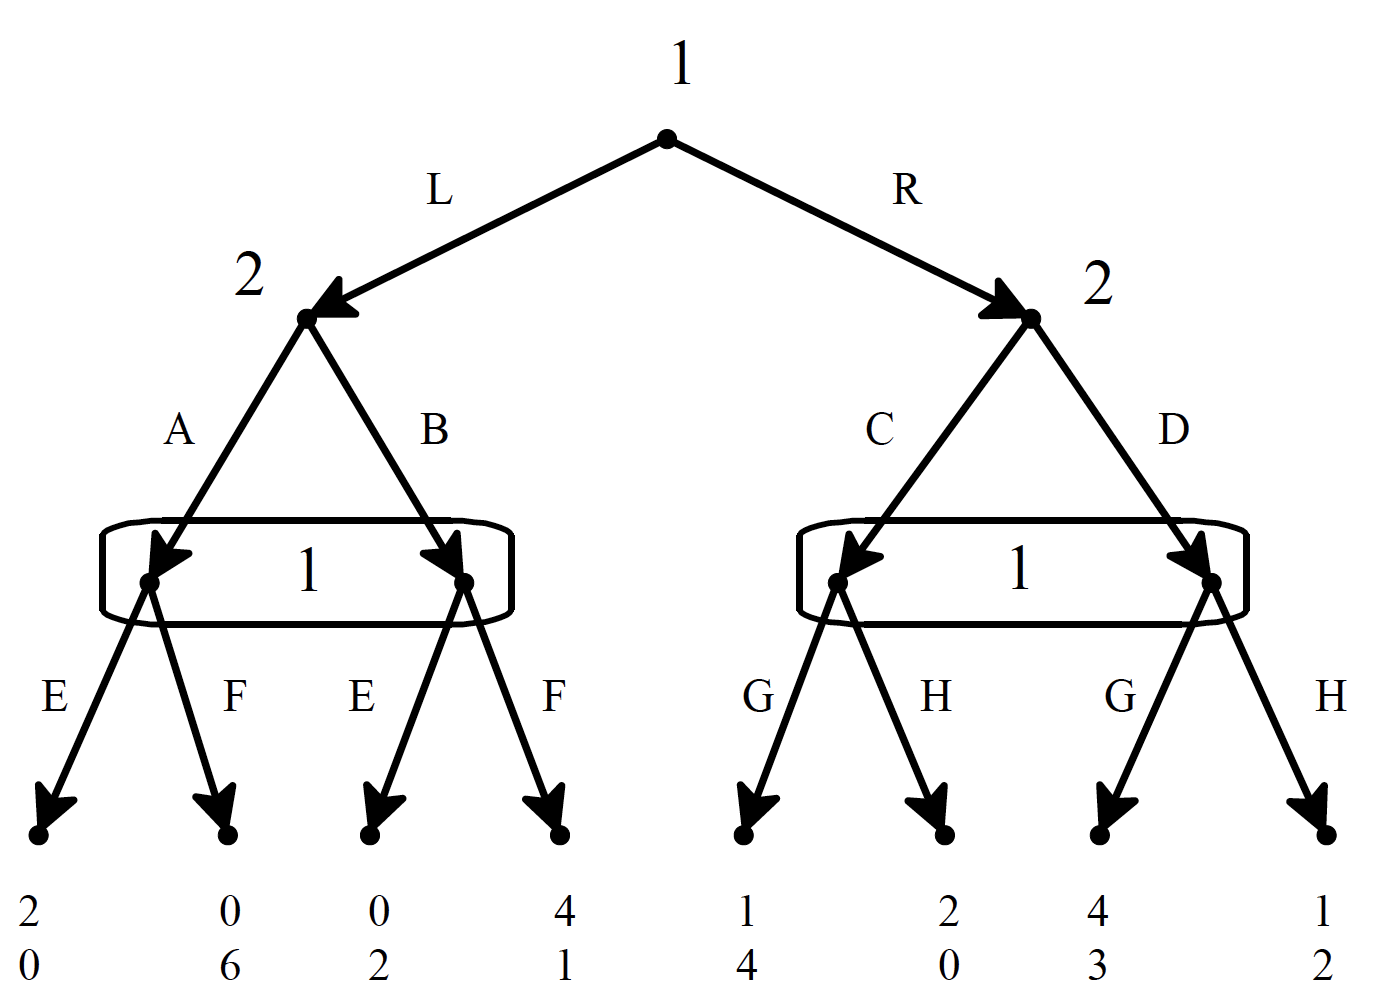
\includegraphics[width=0.5\textwidth,height=\textheight]{exercise7_7.png}

You are asked to answer three questions about it:

\begin{enumerate}
\def\labelenumi{(\alph{enumi})}
\tightlist
\item
  Write the corresponding strategic-form game.
\item
  Find all the pure-strategy Nash equilibria.
\item
  Find the mixed-strategy subgame-perfect equilibrium.
\end{enumerate}

To work out the strategic form, we need to work out everyone's
strategies. Player 1 has three information sets that she plays at - the
top, the bottom left and the bottom-right. And she has two choices at
each of these, so she has \(2 \times 2 \times 2 = 8\) strategies. Player
2 has two information sets that she plays at, and two choices at each,
so she has four strategies. Helpfully, the choices are given different
names, so a string of letters unambiguously names a strategy. Then it is
just a matter of reading off the table to get the payoff table. I'll put
Player 1 on the row, because it is better to have more rows than
columns.

\begin{longtable}[]{@{}ccccc@{}}
\toprule
& AC & AD & BC & BD\tabularnewline
\midrule
\endhead
LEG & 2,0 & 2,0 & 0,2 & 0,2\tabularnewline
LEH & 2,0 & 2,0 & 0,2 & 0,2\tabularnewline
LFG & 0,6 & 0,6 & 4,1 & 4,1\tabularnewline
LFH & 0,6 & 0,6 & 4,1 & 4,1\tabularnewline
REG & 1,4 & 4,3 & 1,4 & 4,3\tabularnewline
REH & 2,0 & 1,2 & 2,0 & 1,2\tabularnewline
RFG & 1,4 & 4,3 & 1,4 & 4,3\tabularnewline
RFH & 2,0 & 1,2 & 2,0 & 1,2\tabularnewline
\bottomrule
\end{longtable}

Now we try to find Nash equilibria by finding best responses. I've
bolded them in this version of the table.

\begin{longtable}[]{@{}ccccc@{}}
\toprule
& AC & AD & BC & BD\tabularnewline
\midrule
\endhead
LEG & \textbf{2},0 & 2,0 & 0,\textbf{2} & 0,\textbf{2}\tabularnewline
LEH & \textbf{2},0 & 2,0 & 0,\textbf{2} & 0,\textbf{2}\tabularnewline
LFG & 0,\textbf{6} & 0,\textbf{6} & \textbf{4},1 &
\textbf{4},1\tabularnewline
LFH & 0,\textbf{6} & 0,\textbf{6} & \textbf{4},1 &
\textbf{4},1\tabularnewline
REG & 1,\textbf{4} & \textbf{4},3 & 1,\textbf{4} &
\textbf{4},3\tabularnewline
REH & \textbf{2},0 & 1,\textbf{2} & 2,0 & 1,\textbf{2}\tabularnewline
RFG & 1,\textbf{4} & \textbf{4},3 & 1,\textbf{4} &
\textbf{4},3\tabularnewline
RFH & \textbf{2},0 & 1,\textbf{2} & 2,0 & 1,\textbf{2}\tabularnewline
\bottomrule
\end{longtable}

And you can see that no cell has two bolded numbers. So there is no
pure-strategy Nash equilibrium.

To find the subgame perfect equilibria, note that the game really boils
down to this game. Player one chooses whether to play this game

\begin{longtable}[]{@{}rcc@{}}
\toprule
& A & B\tabularnewline
\midrule
\endhead
E & 2,0 & 0,2\tabularnewline
F & 0,6 & 4,1\tabularnewline
\bottomrule
\end{longtable}

Or this game

\begin{longtable}[]{@{}rcc@{}}
\toprule
& C & D\tabularnewline
\midrule
\endhead
G & 1,4 & 4,3\tabularnewline
H & 2,0 & 1,2\tabularnewline
\bottomrule
\end{longtable}

Neither game has a pure-strategy Nash equilibrium, so we apply the
formula for finding the equilibrium for finding mixed strategy
equilibria. That gives us for the first game

\[
\Pr(A) = \nicefrac{2}{3}; \Pr(B) = \nicefrac{1}{3}
\] \[
\Pr(E) = \nicefrac{5}{7}; \Pr(F) = \nicefrac{2}{7}
\] \[
V(E) = V(F) = \nicefrac{4}{3}
\]

And for the second game

\[
\Pr(C) = \nicefrac{3}{4}; \Pr(D) = \nicefrac{1}{4}
\] \[
\Pr(G) = \nicefrac{2}{3}; \Pr(H) = \nicefrac{1}{3}
\] \[
V(G) = V(H) = \nicefrac{7}{4}
\]

So player 1, who gets to choose, plays R, then mixes G and H with
probabilities \(\nicefrac{2}{3}\), while player 2 plays C and D with
probabilities \(\nicefrac{3}{4}\) and \(\nicefrac{1}{4}\) respectively.
And they are disposed to use the probabilities above for A, B, E and F
should player 1 play L.

Now imagine a variant on the game. Imagine the payoffs for L-B-F is 4,7
rather than 4,1. What change does this make to the game? First, let's do
the table. I'll just do one table rather than doing one then bolding it.

\begin{longtable}[]{@{}ccccc@{}}
\toprule
& AC & AD & BC & BD\tabularnewline
\midrule
\endhead
LEG & \textbf{2},0 & 2,0 & 0,\textbf{2} & 0,\textbf{2}\tabularnewline
LEH & \textbf{2},0 & 2,0 & 0,\textbf{2} & 0,\textbf{2}\tabularnewline
LFG & 0,6 & 0,6 & \textbf{4},\textbf{7} &
\textbf{4},\textbf{7}\tabularnewline
LFH & 0,6 & 0,6 & \textbf{4},\textbf{7} &
\textbf{4},\textbf{7}\tabularnewline
REG & 1,\textbf{4} & \textbf{4},3 & 1,\textbf{4} &
\textbf{4},3\tabularnewline
REH & \textbf{2},0 & 1,\textbf{2} & 2,0 & 1,\textbf{2}\tabularnewline
RFG & 1,\textbf{4} & \textbf{4},3 & 1,\textbf{4} &
\textbf{4},3\tabularnewline
RFH & \textbf{2},0 & 1,\textbf{2} & 2,0 & 1,\textbf{2}\tabularnewline
\bottomrule
\end{longtable}

Now there are four pure-strategy Nash equilibria. But how many of them
are subgame perfect? Actually, the answer turns out to be none. The
right-hand game is unchanged, so the mixed strategy equilibrium is the
only equilibrium here. But drawing out the left-hand game reveals that
it has a (unique) pure-strategy Nash equilibrium at BF.

\begin{longtable}[]{@{}rcc@{}}
\toprule
& A & B\tabularnewline
\midrule
\endhead
E & 2,0 & 0,2\tabularnewline
F & 0,6 & 4,7\tabularnewline
\bottomrule
\end{longtable}

And now player 1 would get 4 from playing L, so she would prefer that.
The only sub-game perfect equilibrium is that player 1 plays LF, player
2 plays B. But if player 1 had played R, they would have reverted to the
mixed strategy equilibrium.

\hypertarget{extensions-of-subgame-perfection}{%
\section{Extensions of Subgame
Perfection}\label{extensions-of-subgame-perfection}}

Consider again the game from Selten's chain store paradox. The rules are

\begin{itemize}
\tightlist
\item
  First player 2 chooses E for enter or L for leave.
\item
  Then if player 2 chooses E, player 1 chooses C for compete or N for
  normal.
\end{itemize}

The payoff structure is

\begin{itemize}
\tightlist
\item
  If L, the payoffs are 5, 1
\item
  If CE, the payoffs are 0, 0
\item
  If NE, the payoffs are 2, 2
\end{itemize}

And the theoretical point is that the pair E-L is Nash equilibrium, but
not subgame perfect. So far so good. Change the game so that player 2
has three options. If they enter, they can choose to have either Red
uniforms or Green uniforms. This doesn't affect anyone's payoffs, but
player 1 doesn't find out which they chose until after they decide E or
N. Intuitively, this shouldn't change the game, but now the pair E-L is
subgame perfect. (Exercise: why is this?)

So there are a bunch of ideas about how to handle cases like this. The
rough idea is that the following things are all true in equilibrium.

\begin{itemize}
\tightlist
\item
  At each information set, each player has a plan for what they will
  believe about the other players if that set is reached, and (if it is
  their information set) a plan about what to do should they get there.
\item
  The plan about what to do will maximise expected utility given their
  planned beliefs.
\item
  The plan about what to do could be probabilistic - it could be a mixed
  strategy.
\item
  In equilibrium, everyone's (planned) beliefs mesh with everyone else's
  (planned) actions. So if I plan to play A with probability 0.8 and B
  with probability 0.2 at an information set, at that set you belief
  I'll play A with probability 0.8 and B with probability 0.2.
\item
  Everyone's beliefs update in a sensible way. At the very least, if
  something happens that you gave non-zero probability to, then you
  update by conditionalisation. And if something happens that you gave
  zero probability to, then you still believe that everyone has beliefs
  (or probabilities), that they act in ways as to maximise utility given
  their beliefs, that they believe this about everyone else, and so on.
\end{itemize}

That's enough to solve the red uniform/green uniform problem. There is
no way for player 1 to have any beliefs at all about what uniform player
2 has chosen so that C has a higher expected return than N.

But from here on it gets painful. The picture I've sketched so far turns
out to allow equilibria that are not subgame perfect equilibria. So
there becomes a game of finding extra restrictions on how beliefs can
update on probability 0 events to rule that out. But the suggestions for
how to do this are very hard to motivate. So let's stick with what I've
said here, which is roughly weak sequential equilibrium.

\hypertarget{evolutionary-stable-strategies}{%
\section{Evolutionary Stable
Strategies}\label{evolutionary-stable-strategies}}

These only apply to symmetric games. Let's say \(u(x, y)\) is the
utility a player gets from playing \(x\) when the other player does
\(y\). A strategy \(a\) is an evolutionarily stable strategy if for any
other strategy \(b\), either

\begin{itemize}
\tightlist
\item
  \(u(a, a) > u(b, a)\) or
\item
  \(u(a, a) = u(b, a)\) and \(u(a, b) > u(b, b)\)
\end{itemize}

Intuitively, if everyone is playing \(a\), then either playing \(b\)
will do worse, or playing \(b\) will do no better, but then will do
worse if you start running into other \(b\)-players.

One upside of these is that they have a reasonable dynamic alternative.
If you imagine a repeated game between strategies, with the population
at time \(t+1\) proportional to how well that strategy does at time
\(t\), the game tends to some ESS or other.

One related downside is that some ESSs have a very small \textbf{basin
of attraction} - the world has to be just right to end up with them as
the resulting state.

\newpage

\hypertarget{signalling-games}{%
\section{Signalling Games}\label{signalling-games}}

Here is the basic idea of a signalling game.

\begin{itemize}
\tightlist
\item
  There are two players, a sender and a receiver.
\item
  Nature reveals some information to sender. (Or, if you want to make
  the game symmetric, nature chooses one of the two players to reveal
  information to.)
\item
  Sometimes (especially in econonomic applications) we'll call this
  sender's \textbf{type}.
\item
  Sender sends a signal that receiver can see.
\item
  Receiver chooses an action that has a payoff to each player.
\end{itemize}

We'll start by considering \textbf{cooperative} signalling games. These
are games where the players get the same payoff in every situation.
Intuitively, they are ones where the players want to share information
because they are in a joint venture.

To use a famous example, consider Robert Newman, the sexton of the Old
North Church in Boston during the Revolutionary War. Part of his job (as
a revolutionary) was to keep watch for what the Regulars were doing, and
put signals in the window of the church to signal what they were doing.
As the poem says, the signal was ``One if by land, two if by sea''. That
is, he'd put out one lamp if they were coming by land, two if they were
coming by sea. (Actually water; actually the Charles river. But that's
not as poetic.) The other revolutionaries would then take suitable
action.

So here Newman is the sender. Nature (well actually the British army)
has revealed some information to him. (Inadvertently in this case.)
Other people don't know this information. But they do know the signal he
sends; they can see the number of lamps in the window. And they have a
plan for what to do with each thing they see.

Now in reality, the plan they have is a good one. That's because they
have coordinated in advance on what to do. But what if they can't
coordinate. The game in this loose form has any number of Nash
equilibria.

\begin{itemize}
\tightlist
\item
  It has \textbf{separating equilibria} where the townsfolk take
  different actions on seeing the different signals, and things work
  well for hearers and sender.
\item
  It has \textbf{pooling equilibria} where Newman puts up the same
  signal come what may, and the townsfolk do the same thing no matter
  what he does.
\item
  And it has \textbf{babbling equilibia} where Newman chooses randomly
  what to do, and the townsfolk ignore him.
\end{itemize}

But only the separating equilibria are ESS. There are two of these - we
could have had one if by sea, two if by land. But apart from these two
Nash equilibria, the other Nash equilibria are not evolutionarily
stable.

This matters for two big debates

\begin{enumerate}
\def\labelenumi{\arabic{enumi}.}
\tightlist
\item
  What is the relationship between human language and convention?
\item
  How do signalling systems evolve in non-human animals without
  agreement, or in most cases the capacity to do anything like make an
  agreement, as to what the signals will mean?
\end{enumerate}

These are variants of the same question. How do you ever get a
signalling system started? The answer being implicitly suggested here is
that you randomly try a bunch of different strategies for navigating the
world, keep the ones that work and not the ones that don't work (either
intentionally or through natural selection), and eventually you'll end
up signalling. We'll say much more about this over next week.


\end{document}
